\documentclass[a4paper,11pt]{article}
\usepackage[style=mla,style=authoryear,backend=biber]{biblatex}
\renewcommand*{\nameyeardelim}{\addcomma\space}  % add comma between author and year
\usepackage{soul}
\usepackage{hyperref}
\usepackage[colorinlistoftodos]{todonotes}
\usepackage{calc}  % importent in order to import inkspace images
\usepackage[labelfont=bf]{caption}  % set caption label to bold
\usepackage{enumitem}  % to interrupt enumerations and resume
\usepackage{tabularx}  % alternative tabular package for the surveys
\newcolumntype{Y}{>{\centering\arraybackslash}X}  % for centered columns
\usepackage[toc,page]{appendix}

\addbibresource{bibliography.bib}

\graphicspath{ {images/}{graphics/} }

\newcommand{\definition}[1]{\emph{#1}}
\newcommand{\noriinline}[1]{\todo[author=Nori,inline,color=green]{#1}}
\newcommand{\nori}[1]{\todo[author=Nori,color=green]{#1}}
\newcommand{\myunderline}{\rule{2in}{.5pt}}

\title{Audio-Only Augmented Reality System for\\Social Interaction} 
\author{Tom Gurion}

\begin{document}
\maketitle

\listoftodos

\todo[inline]{General question: should I keep general refs to companies, technologies, product etc. in the bibliography or should they present in the footnotes?}

\section{Introduction and framework}

In the past 60 years the development of new technology has fundamentally transformed music creation and consumption (\cite{hargreaves99}).
One of the results of these transformations is interactive music systems (IMS), a concept that faciliting new ways of music creation and blurring the traditional distinction between instrument design, composition and performance (\cite{drummond09}).
In the recent years there are many attempts to provide IMS not only to the professional musicians but also directly accessible to the average user (\cite{stimulant13}).

\todo[inline]{add social context}

Another key concept with high relevance to my work is Augmented Reality (AR).
According to Azuma ``AR enhances a users' perception of and interaction with the real world''.
This concept usually relates to the visual modality: ``AR systems integrate 3-D virtual objects into a 3-D real environment in real time'' (\cite{azuma97}).
My work extend the definition of AR system from the visual to the auditory modality opening the door for more comprehensive experience of virtual environments.

In this work I will combine the concept of IMS with AR creating a system for real-time social interaction for the average user, using current mobile technology.

\section{Literature review}

The current work is based on interdisciplinary research in several different fields.
The following sections will present those fields with emphasis on the projects, technologies and researches that serve as important roots for both my system development as well as the attendant system evaluation.

\subsection{The origins of IMS}

\noriinline{Say that IMS merges development in several threads: early music software, standardization (MIDI), makers community (Arduino, Internet of things)...}

According to the Oxford Dictionary to ``interact'' is to ``act in such a way as to have an effect on each other'' (\citeauthor{web:oxford}).
In the field of IMS actions and affects may be implemented on a broad spectrum of novel techniques, ranging from interactive sound installations to collaborations with robotic performers (\cite{drummond09}).

Since the beginning of the exploration in the field of IMS in the nineteen-sixties, different researchers and composers created systems that were designed to interact with performer in a live situation.
First example of this kind of interactive system was Gordon Mummas' Hornpipe, where specially designed electronic system alters the audio input from the performer and creates an interactive loop between the player and the sound created by the electronics circuit (\cite[p. 12]{winkler01}).

Later, during the nineteen-seventies, musicians and researchers were able to create IMS programmatically using newly developed programming languages designed for musical applications, such as GROOVE or the MUSIC-N series (\cite{mathews70}; \cite{mathews69}).
As a pioneering technology for digital sound synthesis those programming languages gained wide acceptance in the music research community.

On another direction: in the nineteen-eighties a group of musical instruments manufacturers agreed on universal standard for sending and receiving musical information digitally, establishing the MIDI protocol (\cite{web:quinn}).
The standardization of sending and receiving information combined with the emergence of personal computers enabled the creation of modern programing languages for musical applications.
Max/MSP, which began its development by Miller Puckette in 1986, may be a good example (\cite[p. 16]{winkler01}).
As opposed to early programming languages as GROOVE or the MUSIC-N series, most of those personal computer based languages still exist today and keep progressing.
Moreover, new music oriented programing languages are developed on a regular basis, presenting features like ``on-the-fly'' programming (\citeauthor{web:chuck}) or modular, multi-touch environment for live performance (\citeauthor{web:usine}).

Similar technological shifts also facilitated the usage of Digital Audio Workstations (DAW) as a common alternative to analog recording equipment in studios (\cite{leider:04}).
Later, with the arrival of the VST as the common standard for signal processing plug-ins for DAW (\citeauthor{web:steinberg}), computers became even more essential tool for music production.
The arrival of those technologies to the stage could be identified with the emergence of live performance oriented DAW as Ableton Live (\citeauthor{web:live}) and software based DJ setups in late nineteen-nineties.

Another key event in the history of IMS is the appearance of the Arduino platform in 2006.
The Arduino is an easy to use hardware and software package intended for interactive objects or environments creation (\citeauthor{web:arduino}).
The platform opened the door for musicians to use more then just audio and MIDI to communicate with music creation software in interactive environment, mostly by translating physical properties into sound.

More generally, one could see the Arduino as an important part of the new ``Makers'' movements, a technology-based extension of the ``do it yourself'' culture.
The makers, by creating what used to be purchased and by sharing this knowledge back with the community, are a major driving force in the development of IMS nowadays (\cite{web:kirn12}).

\subsection{Interactive music systems for non-professional musicians}

Today, IMS meets the non-professional musician in various scenarios: interactive video clips, mobile and album applications, interactive sound installations and social DJing.
While these examples are typical they are only a small portion of novel ways where non professional can now participate in interactive music creation, interactive consumption of audiovisual content and musically enhanced social interactions.

% interactive video clips: Interlude, Chris Milk and Aaron Koblin
Interactive video clips expose some of the roles traditionally kept for the director to the viewers.
As a relatively new phenomena video clips like those are rare but prominent.
The works by Chris Milk and Aaron Koblin, in which the video clip is run on a dedicated web page and response to the users by tracking their mouse, keyboard strokes or other inputs, can serve as great examples (\citeauthor{web:milk1}; \citeauthor{web:milk2}).
Similar attitude can also be found in the interactive video clips by the startup Interlude (\citeauthor{web:interlude}).

% mobile applications: Smule and RjDj
The increased computation power of the modern mobile phone led developers to develop new mobile applications for music creation for non-professional musicians.
Those applications gives the average user the ability to create music by himself and without any musical education.
Some applications for example: AutoRap turns speech into rap by slicing the syllables and map them according to different beat styles (\citeauthor{web:autorap}); the applications by Brian Eno and Peter Chilvers let users to compose music using only visual element on the device screen (\citeauthor{web:generativemusic}); and RjDj uses the phones' sensors to create ambient sonification based on the users' interactions with the daily environment (\cite{web:rjdj})\label{rjdj}.

% album applications
Album applications are another new trend of artists releasing their music as interactive applications for mobile.
The latest album of the Icelandic musician Bj\"{o}rk, where each song present interactive experience to the user, may be a good example (\cite{stimulant13}).

% interactive sound installations: objects with sound, project ADA
Sound installations are installations located in the three dimensional space that dialog with their surroundings through sound.
Whereas in some interactive sound installations the main interaction is between the viewer and the installation itself (\cite{web:visnjic}; \cite{web:cardiff01}) there are also installations that aims to engage the participants to interact with one another (\cite{eng03}; \cite{web:kirn12}; \cite{web:murray-browne13}).
One may say that the main goal of this later type of installations is to facilitate social interaction.

% social DJing: DistributedDJ, the BLOB and playmysong
Recent projects suggest a framework to share the role of the DJ in a bar or party between the participants (\cite{web:shaw}).
Using those systems participants can choose the music by themselves and the ``playlist'' is generated dynamically by their musical taste.
Most of those project are implemented as mobile applications and some of them even integrate social elements (\citeauthor{web:playmysong}; \cite{web:lammers}).

\subsection{Technology dependent social networking}

Silent disco and flash mobs, the conceptual roots of this research, are examples of modern type of social behavior that rely on the fast growth of social media.
My proposal operates in the context of silent disco party and is inspired by flash mobs in the usage of new technologies to facilitate creative and artistic social interactions.

Silent disco is the phenomenon of partying where the music is heard through headphones instead of loudspeakers.
The new phenomena already changed the possibilities of an ordinary party, for example: having two DJs spin two completely different sets side by side at the same party where each participant has two channel wireless headphones, and can decide which DJ to listen to (\citeauthor{web:headphonedisco}) or having no DJ at all and letting each participant to choose what music to hear, individually, through his or her mobile device and headphones.
Of course, those possibilities are not possible with a regular loudspeaker setup.

Flash mobs is a public gathering of people organized through social media to perform a short and seemingly pointless act and then disperse.
Because of the way flash mobs are organized different researchers see the phenomenon as a significant event in the history of mobile communication (\cite{nicholson05}) and even suggest that it inherently reflects an artistic intent (\cite{brejzek10}).

\subsection{Social effects of music}

% Music as a way for communication.
Music is known for being an important channel of communication.
It provides musicians with the ability to share emotions and meanings without words and can produce deep feelings among listeners (\cite{hargreaves02}).

% Music social function.
% The influence on individual self identity and interpersonal relationships as described by Hargreaves and North.
Throughout the twentieth century the psychological functions of music in everyday life have been extensively studied, with an emphasis on their cognitive and emotional importance for the individual (\cite{hargreaves99}).
A recent study by Hargreaves and North tries to extend those insights about music functionality to the social domain, explaining the social effects of music on the individual by means of self-identity, inter-personal relationships and mood.

% Classification of personality dimensions, self-views and cognitive abilities according to musical preferences as suggested by Rentfrow and Gosling.
In todays world people think and identified themselves through music in such a way that cultural phenomena are often described by the musical style that accompanies them (e.g., the youth generation in the nineteen-sixties) (\cite{cook00}).
Indeed, there is a high correlation between music preferences and a wide array of personality dimensions (e.g., conscientiousness and openness) as well as self-views (e.g., political orientation) (\cite{rentfrow03}).

\noriinline{Some references more general about the cognitive and social aspects. Includes group cohesion, in-group \& out-group. Currently it sounds to me quite shallow}

\subsection{Indoor positioning systems}

\todo[inline]{does the following sentence add something at all?}

The system I propose will require the ability to locate the positioning of the users within an indoor environment.

Today, the usage of outdoor positioning systems is unquestioned and achieved mainly by the General Positioning System (GPS) which is available in almost any modern phone.
On the other hand, IPS has not been standardized yet and therefor it is still not available to the average user (\cite{web:turetsky}).

Recent researches state that WiFi is a favored technology among IPS for mobile devices.
WiFi based systems can also enhance accuracy by applying inertial navigation using additional sensors of the device such as accelerometer, gyroscope, compass etc. (\cite{web:harrop}).
Note however that those solutions depend on the deployment of WiFi infrastructure in every indoor environment where positioning information in desired.

\section{Research targets}

The system developed in this research is inspired by the concepts of IMS and intended for the average user. In this research I will focus on the two following targets:
\begin{enumerate}
	\item To propose and implement an audio-only augmented reality system for social interaction.
	Using the system, participants will be able to interact with one another as well as with systems' components and affect the structure of the music in a virtual space.
	\item To evaluate the social effects of the system usage in the context of a silent disco party mainly focusing thereby on the following research question: \emph{Does the system elaborate social interaction between participants in an interactive silent disco party?}
\end{enumerate}

\section{Research methods}

\subsection{System development}

In this section I will explain the rational for the choices of system implementation in the context of the above research targets.

\subsubsection{Mobile and Android}

Todays' mobile phone has transformed from being a simply communication tool into a key `social object' in everyday life, and as such it has a significant importance in shaping todays' society (\cite{srivastava05}).
The applications of this research are targeted for the general audience and therefor the entire research will be implemented for mobile.

The system will be developed for the Android operation system (\citeauthor{web:android}).
Choosing Android as the platform for my research has two main advantages:
\begin{enumerate}
	\item The Android system is a growing mobile system which controls most of the market share today (\cite{web:idc}).
	\item By developing application for Android I have access to underlying Bluetooth properties such as received signal strength indicator (RSSI), which is essential for my implementation of the system as laid out in the next section.
\end{enumerate}

\subsubsection{Indoor positioning system}\label{methods:ips}

Although there are available techniques to implement IPS I have decided to develop one by my own.
This decision has been done due to three reasons:
\begin{enumerate}
	\item Most of the techniques available nowadays require infrastructure.
	As a system influenced by flash mobs I wanted to be able to use it anywhere without the effort involved in infrastructure deployment.
	\item Tracking the positioning of the participants as well as the positioning of the balloon bundles has a lot of overhead when the only requirement is to be able to approximate the distance between each participant and his surrounding bundles.
	\item As opposed to system where high accuracy is required, the current research does not demand it.
	Being able to estimate if a participant is relatively close to a beacon or far from it is generally satisfying.
\end{enumerate}

The system I have developed --- the Bluetooth Based Relative Indoor Positioning (BBRIP) system --- consists of some Bluetooth beacons, placed inside the balloon bundles, and an Android application.
It is build around distributed architecture and therefor runs separately, as an Android application, on each one of the participants phones.
The application repeatedly searches for nearby Bluetooth beacons.
Received signal strength indication (RSSI) is used as an estimation of the distance between the user and the beacon.

\subsubsection{libpd}\label{methods:libpd}

Advance audio processing is beyond the capabilities of the Android application programming interface and therefor, in order to apply sophisticate manipulations on the audio in real time, a more powerful audio engine was required.
In a personal computer environment the programming language Pure Data (Pd), originally written by Miller Puckette in the nineteen-nineties, is one of the leading open-source softwares for computer music (\citeauthor{web:pd}).
In this research I have decided to use ``libpd'', a thin layer on top of Pd that turns it into an embeddable audio library, as an audio engine (\cite[p. v]{brinkmann12}).

\subsubsection{System description}\label{systemdescription}

\begin{figure}[!htb]
	\centering
	\def\svgwidth{0.9\textwidth}
	\input{graphics/system_architecture.pdf_tex}
	\caption{System architecture}\label{fig:sys:architecture}
\end{figure}

Figure \ref{fig:sys:architecture} shows a schematic diagram of the system, which consist of an Android application and specially designed Bluetooth ($BB1 - BB4$).
The BBRIP system is used to estimate the distance between the user and nearby Bluetooth beacon.
This estimation is then sent to a Pd patch through libpd, which plays an audio loop corresponding to the nearby beacon by one of the sound zone players $SZP1$ -- $SZP4$.
Every audio loop is identified by a distinct musical style which can be rhythmically and harmonically synchronized with other loops in almost endless combinations.

\begin{figure}[!htb]
	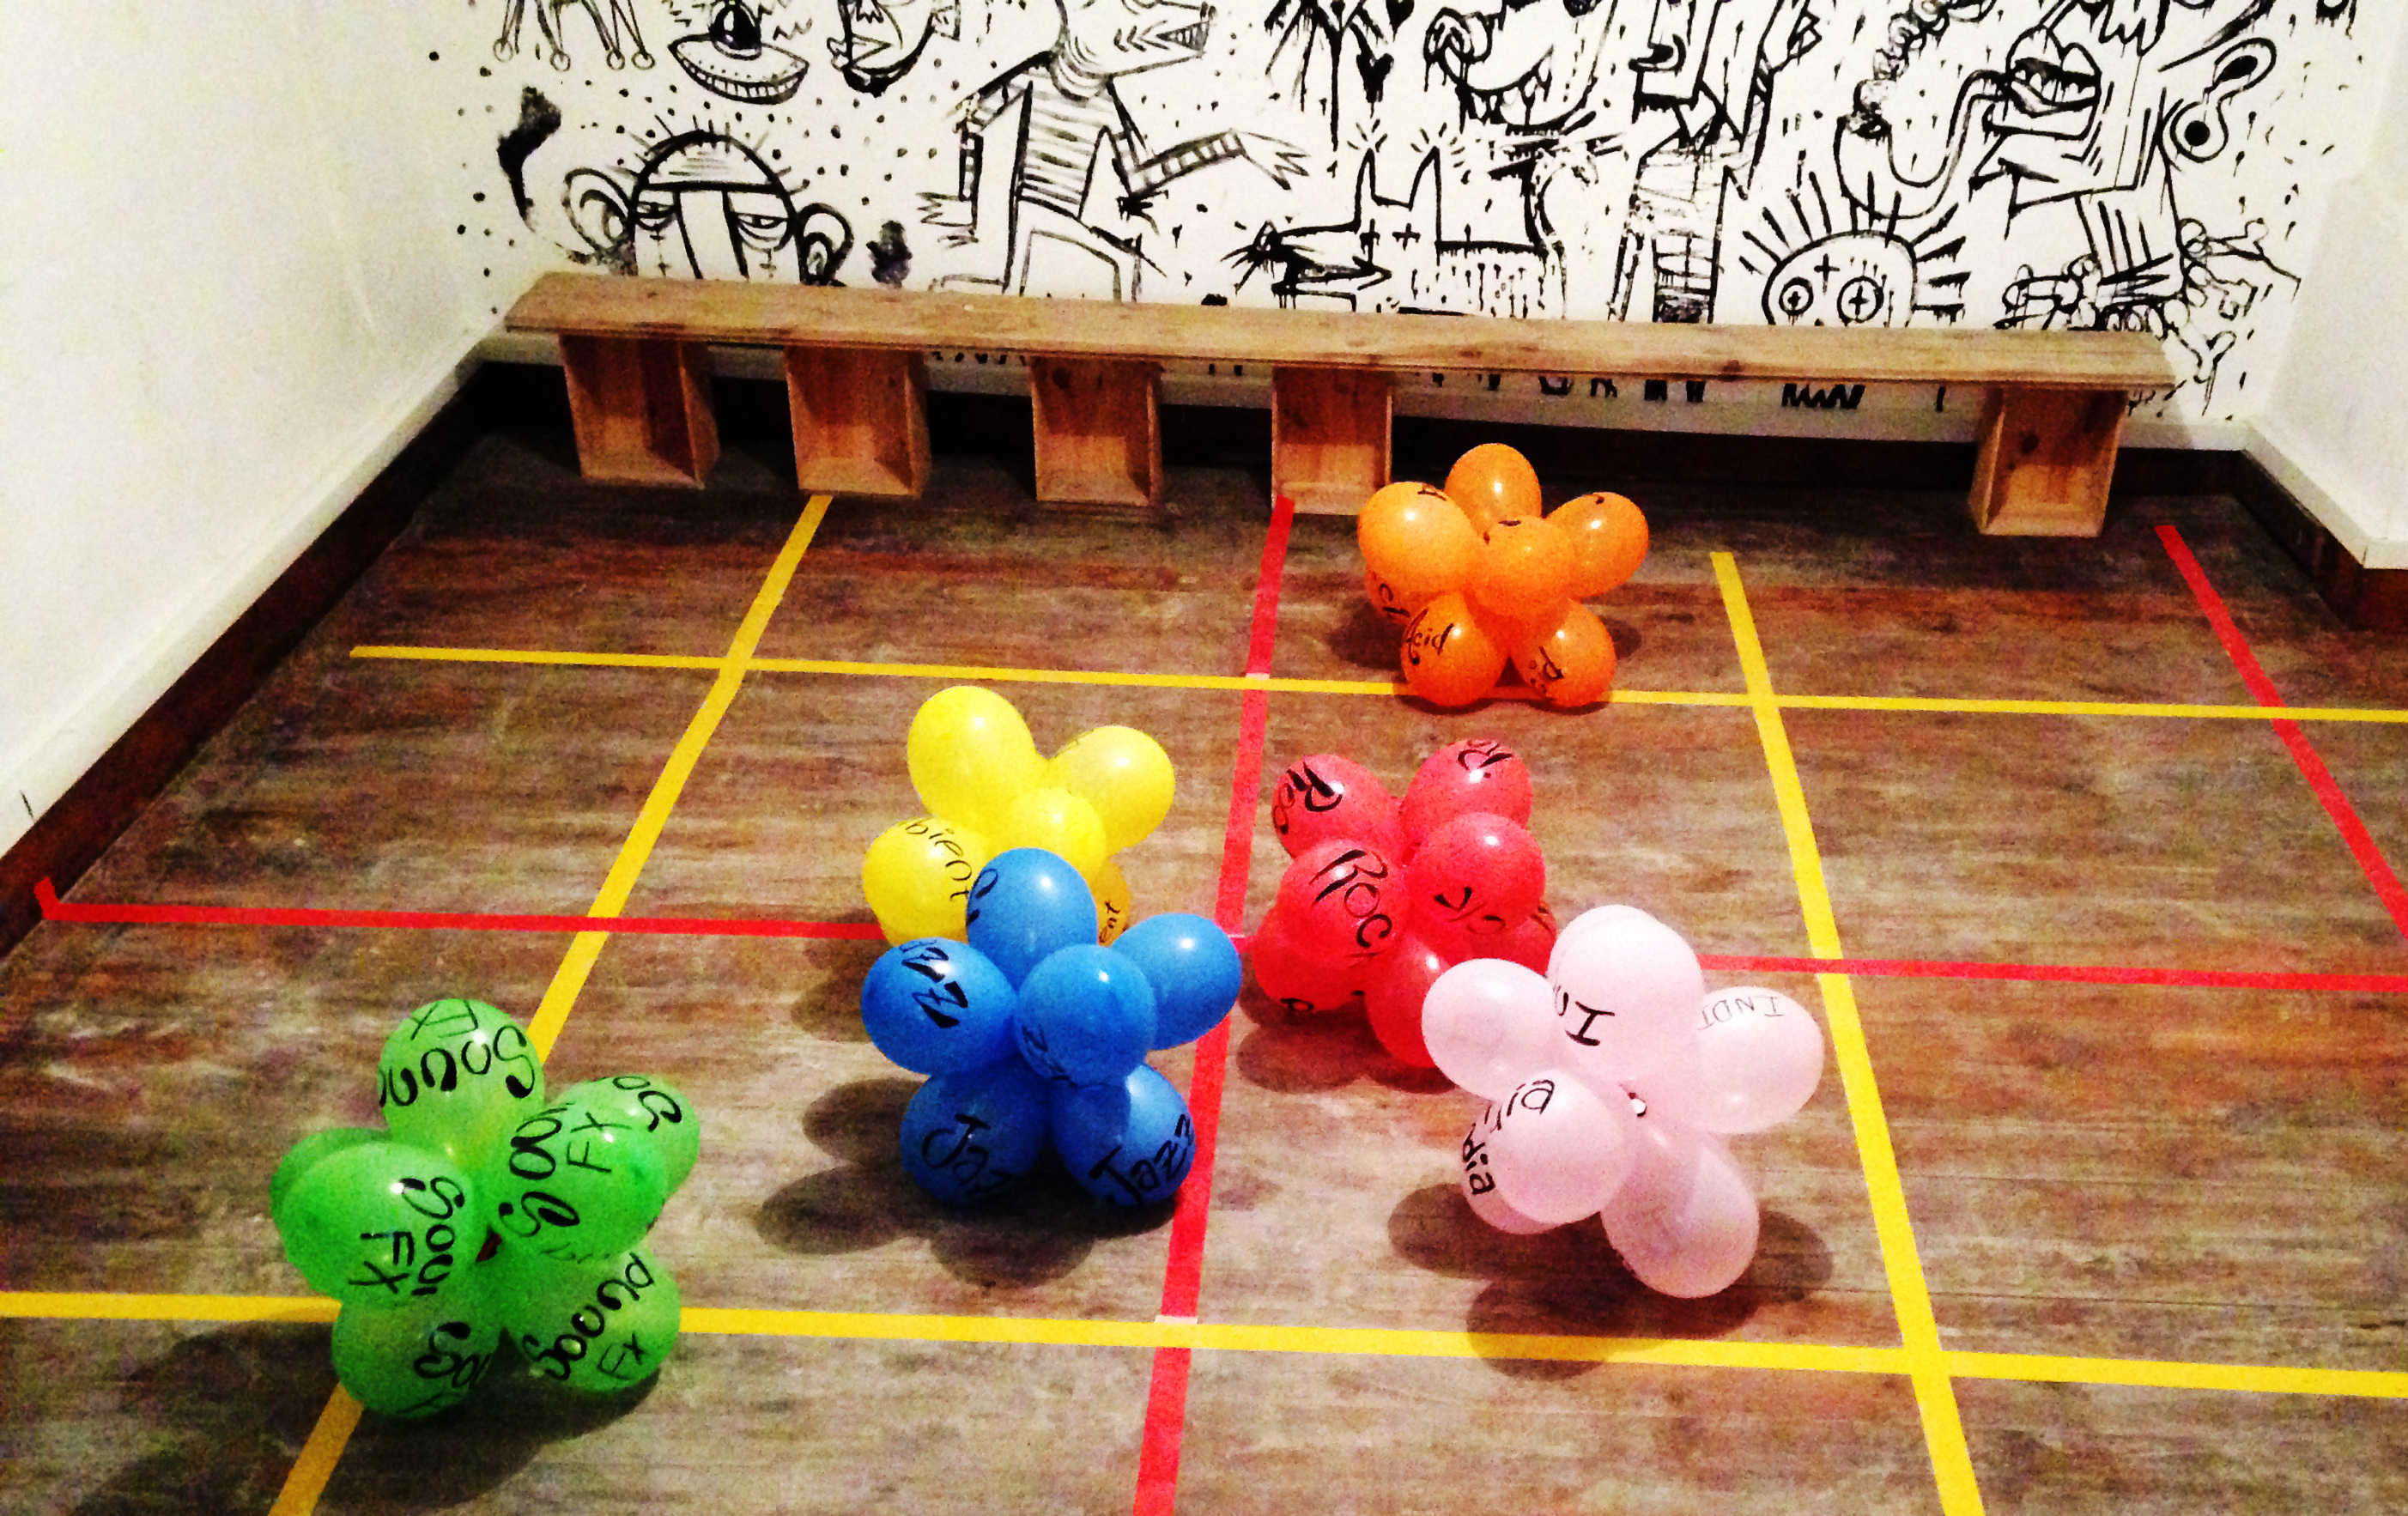
\includegraphics[width=\linewidth]{balloons}
	\caption{Balloon bundles on the dance floor}\label{fig:balloons}
\end{figure}

From the participants point of view the dance floor will consist of few balloon bundles, each one marked up with a name of specific musical style (e.g.\ rock, jazz, Indian music as shown in figure \ref{fig:balloons}).
A corresponding Bluetooth beacon will be installed inside each one of those bundles.
After downloading and installing the Android application, strolling between the balloon bundles will affect the music in ones headphones according to the relative distance from the bundles, creating a virtual ``sound zone'' around each one of them.
In addition, the distance from the center of each sound zones may affect the music in several different ways; for example by controlling volume, filter and granularity of the sound zone.
Lastly, participants can freely move the balloon bundles, thereby changing the structure of the music in the virtual space making it socially interactive.

Figure \ref{fig:sys:participant_view} shows an overhead view of a possible scenario of participants using the system in a party\footnote{A video demonstration of similar scenario can be found at \href{http://youtu.be/2kJoeD2iWBA}{youtu.be/2kJoeD2iWBA}.}.

\begin{figure}[!htb]
	\centering
	\def\svgwidth{0.9\textwidth}
	\input{graphics/system_participant_view.pdf_tex}
	\caption{Here you can see two participants, $A$ and $B$, dancing around three Bluetooth beacons, corresponding to the rock, jazz and Indian music sound zones. Participant $A$ hear rock music and participant $B$ hear a mix between the jazz and the Indian music sound zones, which are rhythmically and harmonically synchronized with each other.}\label{fig:sys:participant_view}
\end{figure}

\subsection{System evaluation}\label{methods:evaluation}

A controlled experiment will be conducted in order to asses the research question: \emph{Does the system elaborate social interaction between participants in an interactive silent disco party?}

\subsubsection{Participants}

Thirty undergraduate and graduate-level students from the Music Department of Bar-Ilan university will participate in the experiment.
Their participation will rely on voluntarily will.

\subsubsection{Measurements}

The above research question will be fragmented into the following operational definitions and measurements\footnote{Complete version of each of the surveys below can be found in the appendix.}:
\begin{enumerate}
	\item \label{measure:disperse} Assuming that participants are pre-partitioned, natively, as groups of friends, we can define the \definition{momentary center} of each group as the average positioning of its participants on the two dimensional plain of the dance floor.
	In addition, we can define the \definition{momentary disperse} of each group as the variance of its participants' positionings around the center\footnote{Two dimensional variance definition is presented in the appendix.}.
	Using the above definitions interaction between the members of one group with other participants will be evaluated by the disperse of the groups, when high disperse values indicate higher interactivity.
	\item \label{measure:groups} Using the above definitions, we can define \definition{momentary group disperse} as the variance of the momentary centers themselves on the dance floor.
	With this regards low momentary group disperse values indicate higher interactivity.
	\item \label{measure:audio} The audio volume inside the experiment room will be used as an indication for the amount of `speaking' between participants and therefor as a social interaction estimation.
	\item \label{measure:survey:social} Participants will fill social interaction survey.
	The survey will be used to asses interaction between participants by estimating social cohesiveness within in-group and out-group of each participant.
\end{enumerate}
In addition to measurements intended to assess the main research question.
The following operational definitions and measurements will be used in order to assess interaction with and satisfaction from the system.
\begin{enumerate}[resume]
	\item \label{measure:system} We will define \definition{momentary participant-system interaction} as the momentary distance of each participant from the closest Bluetooth beacon.
	Using the above definition high level of interaction of participant with the system will be indicated by low values of momentary participant-system interaction.
	\item \label{measure:survey:usability} Participants will fill system satisfaction survey, based on the System Usability Scale (\cite{brooke96}).
\end{enumerate}
Lastly, the following measurement will be used in order to eliminate possible differences between research groups and to allow future research based on the retrieved data.
\begin{enumerate}[resume]
	\item \label{measure:survey:musical} Participants will fill musical background survey, based on the Emmanuel College Music Background Questionnaire, basic version (\cite{web:zhao12}).
\end{enumerate}

\subsubsection{Apparatus}

In order to measure momentary disperse and group disperse as defined in measurements \ref{measure:disperse} and \ref{measure:groups} I will capture the experiment with video camera from above the dance floor.
Tracking the positioning of the participants will be done half manually by using software aids to record the manual tracking of participants, each at a time, using the computer mouse.
The results will be then processed using computational programming to conclude insights from the data.

Tracking data required in order to compute momentary participant-system interaction, as described in measurement \ref{measure:system}, will be derived the same way, by manually tracking each one of the system components in the video.

Audio volume (measurement \ref{measure:audio}) will be captured by a microphone and analyzed afterwards.

\subsubsection{Procedure}

Participants will be randomly allocated into two groups, group $A$ and group $B$\@.
Each group will participate in the experiment in different week, but in the same day of the week and same hour.

\begin{figure}[!htb]
	\centering
	\def\svgwidth{0.8\textwidth}
  	\input{graphics/procedure.pdf_tex}
	\caption{Experiment design}\label{fig:experiment}
\end{figure}

Participants will first fill a musical background survey as described in measurement \ref{measure:survey:musical}, followed by three \definition{experiment blocks}, followed by a system usability survey as described in measurement \ref{measure:survey:usability} (see figure \ref{fig:experiment}).
Each experiment block will consist of 15 minutes in which participants listen to music in their headphones, using their Android device and pre-installed application, and interact with other participants in the `silent disco' party.
Meanwhile, during each experiment block, measurements \ref{measure:disperse}, \ref{measure:groups}, \ref{measure:audio} and \ref{measure:system} will be collected.
Before each experiment block and after the last block each participant will fill the social interaction survey (measurement \ref{measure:survey:social}).

Each experiment block can be of one of the following types:
\begin{description}
	\item[Interactive:] In which the music generated by the Android application behaves as described in chapter \ref{systemdescription}.
	\item[Control:] In which the music generated by the Android application is pre-composed and based on the same musical materials as of the interactive system.
\end{description}

Participants of group $A$ will hear the experiment blocks: Control $\rightarrow$ Interactive $\rightarrow$ Control. Whereas participants of group $B$ will hear the experiment blocks: Control $\rightarrow$ Control $\rightarrow$ Control.

\todo[inline,color=red]{reasoning for the design is missing}

\section{Preliminary results}

\subsection{System development}

The system development could be described by two different processes: the development of the BBRIP system and the Android application that wraps it and is responsible for the audio processing.

\subsubsection{Implementation of the BBRIP system}

The BBRIP system is my intent to develop an indoor positioning system that will satisfy the relatively simple requirements of the research as presented in chapter \ref{methods:ips}.
As already noted, such a solution not yet exist.

My implementation of the system is based on a specific element in the Bluetooth protocol -- the Received Signal Strength Indicator (RSSI) ({\cite{bray12}).
Each Bluetooth enabled device calculate RSSI values during Bluetooth discovery, when it finds a new device and before establishing connection.

\begin{figure}[!htb]
	\centering
	\def\svgwidth{\columnwidth}
  	\input{graphics/bbrip.pdf_tex}
	\caption{The BBRIP system}\label{fig:bbrip}
\end{figure}

As shown in figure \ref{fig:bbrip}, the BBRIP system continuously search for Bluetooth devices.
When a new device is found the RSSI value is extracted and send forward for processing.
From the first discovery in the Bluetooth discovery cycle the system keeps checking if the time since the last discovery exceeded a pre-defined timeout and if so it terminate the discovery.
This termination is important because naturally a device can only be discovered once in each Bluetooth discovery cycle and long period of time without new discoveries indicates that all of the nearby devices are already found.
Lastly, when the system sees that there is no Bluetooth discovery running (because of termination or simply the end of the discovery cycle), it starts a new one immediately.

Although the RSSI values extracted by the BBRIP system are not very precise as a distance estimation, I have found them sufficient enough in order to classify the distance between participants and beacons into useful ranges. In other words, RSSI values gives great indication if a participant is stands close to specific beacon (around 1 meter), in mediate range (2 to 3 meters) or in larger distance.

\subsubsection{ScenePlayer Plus}

The development of the Android application moved through different development stages.

First, I have developed an application that didn't use ``libpd'' at all (see chapter \ref{methods:libpd}).
In this early stage the only effect of getting close to, or far from a beacon was by changing the volume.
In addition, the limited sophistication of the built in audio library made fading in and out from the sound zones very non-flexible.

After finding the weakness of using the built in audio library of the Android application programming interface I have decided to implement the system using ``libpd''.
Although this implementation worked fine, it made a very tight coupling between the system development in the Android environment and the audio processing development in Pd.
Overall, this development phase was sufficiant enough but in order to allow other musicians and developers to use the system I have started to look for more open architecture, that will maintain loosely coupled connection between the Android application and the Pd patch that drove the audio.

The last phase in the development of the system was to implement the BBRIP system into the open source Android application ``ScenePlayer'' (\cite{web:sceneplayer}), an Android port for the RjDj application mentioned in chapter \ref{rjdj}, and release it again as ``ScenePlayer Plus'' (\cite{web:sceneplayerplus}).
The application exposes the Bluetooth RSSI values to the Pd patch as another sensor of the mobile device (e.g. accelerometer, compass and touchscreen).

\subsection{System evaluation}

The following describe a pilot experiment I have run, with different methods then those presented in chapter \ref{methods:evaluation}.

\subsubsection{Pilot experiment design}

\begin{figure}[!htb]
	\centering
	\def\svgwidth{0.95\columnwidth}
  	\input{graphics/pilot_design.pdf_tex}
	\caption{Pilot experiment design}\label{fig:pilot}
\end{figure}

Eighteen volunteers was invited to participate in an interactive silent disco party.
Each participant installed the Android application on his or her phone and filled pre/post party surveys that included questions regarding their musical background and preferences as well as system evaluation feedback.
The party consisted of four alternating interactive/control blocks of duration 5:40 minutes each (see figure \ref{fig:pilot}).
The participants were randomly assigned to two groups: $A$ and $B$, comprising the interactive and control blocks respectively\footnote{Group $A$ (interactive first) consists of 8 participants (4 females and 4 males) with mean age of 36.7 (s.d=12.3); group $B$ (control first) consists of 10 participants (3 females and 7 males) with mean age of 29.6 (s.d=10.2). Participants had a diverse musical background with 4.7 mean years of musical training (s.d=5.2).}.
They were generally informed that the experiment consists of interactive and control segments, however they were not informed about the exact schedule and timing of the blocks or the group assignments.
Both groups started the experiment together.
In the interactive blocks, the application generated music as described in chapter \ref{systemdescription}, whereas in the control blocks the participants heard recorded non-interactive music created in advance using the musical material of the interactive system\footnote{The control block music composed by Noam Elron (\href{http://www.noamelron.com}{www.noamelron.com}).}.

Interaction with the systems' components was assessed by counting the number of Bluetooth device discoveries made by each participants' phone during both the interactive and the control blocks.
In order to eliminate edge effects, we analyzed only the two middle blocks of the experiment.

\subsubsection{Pilot experiment results}

\begin{figure}[!htb]
\minipage{0.49\textwidth}
	\def\svgwidth{0.95\columnwidth}
  	\input{graphics/changing_location_in_space.pdf_tex}
	\caption{Changing location in space}\label{fig:location}
\endminipage\hfill
\minipage{0.49\textwidth}
	\def\svgwidth{0.95\columnwidth}
	\input{graphics/dancing_with_known_people.pdf_tex}
	\caption{Dancing with known people}\label{fig:known}
\endminipage\hfill
\end{figure}

In the post-party survey, participants self-reported significantly higher levels of movement (paired t-test, $t(15)=3.9$, $p<0.01$) using the system, compared with their behavior on other parties as reported in the pre-party survey.
Figure \ref{fig:location} shows that there was a significant difference (unpaired t-test, $t(33)=6.2$, $p<0.01$) in the mean response to these questions (at a scale of 1-3).

In order to objectively assess if participants moved more in space, we measured the counting of Bluetooth discoveries made by the applications' BBRIP system.
The results show slightly higher counts (paired t-test, $t(16)=1.7$, $p=0.06$, n.s) during the interactive blocks of the party compared with the control blocks. This suggests that the interactive components of the system facilitate greater participant movement in space, thereby offering more frequent opportunities for social interactions.
Indeed, in the post-party survey participants reported that they danced significantly less with people that they knew in advance, compared with their usual behavior (paired t-test, $t(14)=-2.5$, $p=0.01$).
Figure \ref{fig:known} shows that there was also a significant difference in the mean response to these questions in the pre/post surveys.
Overall, participants showed a slightly stronger tendency (paired t-test, $t(16)=1.46$ ,$p=0.08$, n.s) to participate in an interactive party in the post-party survey, compared with their answer to identical questions in the pre survey.

The preliminary results already demonstrate the potential for audio-only augmented reality to significantly enrich the experience of music consumption and its attendant social interaction.
We also show that this can be validated in a controlled experiment using both direct reports of subject and indirect objective measurements.

More generally, my research explores the potential for using modern technologies to create IMS for non-professional musicians, where the user' social interaction is the main influence over actually heard music.

\begin{appendices}

\todo[inline,color=red]{write interaction survey!}
\todo[inline]{write 2d variance}

\section[Musical background survey]{Musical background survey\\
	{\normalsize based on the Emmanuel College Music Background Questionnaire, basic version}}

Please first provide your basic information.

\begin{enumerate}
	\item Name: \myunderline
	\item Gender: Male / Female
	\item Age: \myunderline
	\item E-mail: \myunderline
\end{enumerate}
Please answer the following questions to the best of your knowledge.
\begin{enumerate}[resume]

	\item Please rate your overall interest in Music according to the following scale

	\begin{tabular}{c c c c c}
		Not interested & & Neutral & & Very interested \\
		1 & 2 & 3 & 4 & 5 \\
	\end{tabular}

	\item Please rate your overall Music ability according to the following scale

	\begin{tabular}{c c c c c}
		Poor & & Average & & Excellent \\
		1 & 2 & 3 & 4 & 5 \\
	\end{tabular}

	\item How many hours per week do you spend listening to music?

	\myunderline

	\item What genre(s) do you listen to most? (check all that apply)

	\begin{tabular}{l l}
		{[{ \ }]} & Classical \\
		{[{ \ }]} & Country \\
		{[{ \ }]} & Jazz \\
		{[{ \ }]} & Rock \\
		{[{ \ }]} & Pop \\
		{[{ \ }]} & Non-western \\
		{[{ \ }]} & Other: (please specify) \myunderline \\
	\end{tabular}

	\item Most of the time, when you listen to music, you are

	\begin{tabular}{l l}
		( \ ) & not focused on the music, attending to a different task \\
		( \ ) & passively listening \\
		( \ ) & highly aware of musical nuances such as key changes, harmonies, etc. \\
		( \ ) & actively engaged (sing along, tap the beat, etc.) \\
	\end{tabular}

	\item About how many hours of musical activity do you engage in each week currently? (e.g. practice, performance)

	\myunderline

	\item \label{appendix:music:ensamble}Have you ever participated in a musical ensemble?

	\begin{tabular}{l l}
		( \ ) No \\
		( \ ) Yes, instrumental ensemble \\
		( \ ) Yes, vocal ensemble \\
		( \ ) Yes, both instrumental and vocal \\
	\end{tabular}

	\item If you answered YES to question \ref{appendix:music:ensamble}, please indicate how many years you have participated in the music ensemble

	\myunderline \ years

	\item Please list any instrument(s) that you play (including voice) and the years you play each of them, beginning with your primary instrument:

	\begin{tabular}{c c}
		Instrument &  Years playing \\
		\myunderline & \myunderline \\
		\myunderline & \myunderline \\
		\myunderline & \myunderline \\
		\myunderline & \myunderline \\
	\end{tabular}
	
	\item \label{appendix:music:before_break}Have you ever had any formal training in music? (If you are a self-taught musician, please also answer YES)

	\begin{tabular}{l l}
		( \ ) & YES, I had a formal training in music \\
		( \ ) & YES, I consider myself a self-taught musician \\
		( \ ) & NO \\
	\end{tabular}

\end{enumerate}
Please continue this form if you answered YES to question \ref{appendix:music:before_break}, otherwise please go directly to question \ref{appendix:music:after_break}.
\begin{enumerate}[resume]

	\item What type(s) of music training have you had? (check all that apply)

	\begin{tabular}{l l}
		{[{ \ }]} & private/small group lessons in instrument and/or voice \\
		{[{ \ }]} & institutional training \\
		{[{ \ }]} & University degree in music - list degree: \\
		{[{ \ }]} & self-taught \\
		{[{ \ }]} & other (please specify): \myunderline \\
	\end{tabular}

 	\item At what age did you begin to study music?

 	\myunderline

 	\item How long did your formal music training last?

 	\myunderline \ years
 	\item How long has it been since you last participated in formal music lessons?

	\begin{tabular}{l l}
		( \ ) & Currently have one \\
		( \ ) & Or \myunderline \ years \\
	\end{tabular}

	\item \label{appendix:music:after_break}If there is anything else that you feel is interesting or important about your musical background, please comment below:

	\rule{4.5in}{.5pt} \\
	\rule{4.5in}{.5pt} \\
	\rule{4.5in}{.5pt} \\
	\rule{4.5in}{.5pt}.

\end{enumerate}

\section[System satisfaction survey]{System satisfaction survey\\
	{\normalsize based on the System Usability Scale}}

\begin{tabularx}{\textwidth}{p{2in} | Y Y Y Y Y }
	& Strongly disagree & & & & Strongly agree \\
	\hline
	I think that I would like to use this system frequently & 1 & 2 & 3 & 4 & 5 \\
	\hline
	I found the system unnecessarily complex & 1 & 2 & 3 & 4 & 5 \\
	\hline
	I thought the system was easy to use & 1 & 2 & 3 & 4 & 5 \\
	\hline
	I think that I would need the support of a technical person to be able to use this system & 1 & 2 & 3 & 4 & 5 \\
	\hline
	I found the various functions in this system were well integrated & 1 & 2 & 3 & 4 & 5 \\
	\hline
	I thought there was too much inconsistency in this system & 1 & 2 & 3 & 4 & 5 \\
	\hline
	I would imagine that most people would learn to use this system very quickly & 1 & 2 & 3 & 4 & 5 \\
	\hline
	I found the system very cumbersome to use & 1 & 2 & 3 & 4 & 5 \\
	\hline
	I felt very confident using the system & 1 & 2 & 3 & 4 & 5 \\
	\hline
	I needed to learn a lot of things before I could get going with this system & 1 & 2 & 3 & 4 & 5 \\
	\hline
\end{tabularx}

\end{appendices}

\sloppy  % fixing line breaks in bibliography
\printbibliography[title={Bibliography}]
\end{document}